\chapter{Эксперименты}

\section{Кросс валидация}
Так как в нашем распоряжении было не много размеченных данных, для исключения
переобучения использовалась кросс валидация. Как было описано ранее, предметным
специалистом были предоставлены примерно одинаковые по продолжительности записи
с разных экспериментов, в связи с чем было логично сделать разбиение на группы
именно по ним. Таким образом, всего получилось 8 групп --- по 1 на
валидацию и тестирование и по 6 на обучение. Всего производилось 8
экспериментов (по одному на уникальную тестовую группу). Валидационная группа
выбиралась случайным образом. Метрики замерялись после обучения на тестовой
группе. В качестве финальной метрики бралось среднее от всех экспериментов.

\section{Результаты}

В определенный момент времени возникла потребность в ручной проверке и
корректировке истинной разметки. Таким образом, у нас появилась более
качественная разметка, на основе которой были измерены метрики. В таблице
\ref{tab:results} показано сравнение результатов работы двух программ: той,
которая описана в данной работе, и той, с помощью которой был выполнен
первоначальный анализ. Для более наглядного сопоставления приведен график
итоговой метрики F1-score на рис. \ref{fig:f1score-vs}.

Как показывает сравнение, удалось достичь повышения качества работы на 11\%,
причем данный подход отличается от оригинальной программы тем, что полностью
автоматизирован и не требует тонкой настройки специалистом.

\begin{table}[ht]
	\centering
	\label{tab:results}
	\begin{tabular}{ccccccc} \toprule
		                     & \multicolumn{2}{c}{Precision} & \multicolumn{2}{c}{Recall} & \multicolumn{2}{c}{F1-score}                                        \\
		\textbf{Эксперимент} & \textbf{O}                    & \textbf{P}                 & \textbf{O}                   & \textbf{P} & \textbf{O} & \textbf{P} \\ \midrule
		22ph0 & 0.99 & 0.99 & 0.98 & 0.99 & 0.99 & 0.99 \\
		22ph1 & 0.98 & 0.71 & 0.45 & 0.93 & 0.62 & 0.81 \\
		23ph0 & 0.98 & 0.98 & 0.89 & 0.97 & 0.93 & 0.97 \\
		23ph1 & 0.96 & 0.85 & 0.38 & 0.64 & 0.55 & 0.73 \\
		25ph0 & 0.96 & 0.75 & 0.85 & 0.99 & 0.90 & 0.86 \\
		25ph1 & 0.37 & 0.78 & 0.85 & 0.94 & 0.52 & 0.85 \\
		26ph0 & 0.99 & 0.84 & 0.71 & 0.97 & 0.83 & 0.90 \\
		26ph1 & 0.99 & 0.58 & 0.38 & 0.87 & 0.55 & 0.70 \\ \midrule
		\textbf{Среднее} & 0.90 & 0.81 & 0.69 & 0.91 & 0.74 & 0.85 \\
		\bottomrule
	\end{tabular}
	\caption{\centering Результаты экспериментов. O --- оригинальная разметка, P --- предсказанная}
\end{table}

\begin{figure}[!htb]
	\centering
	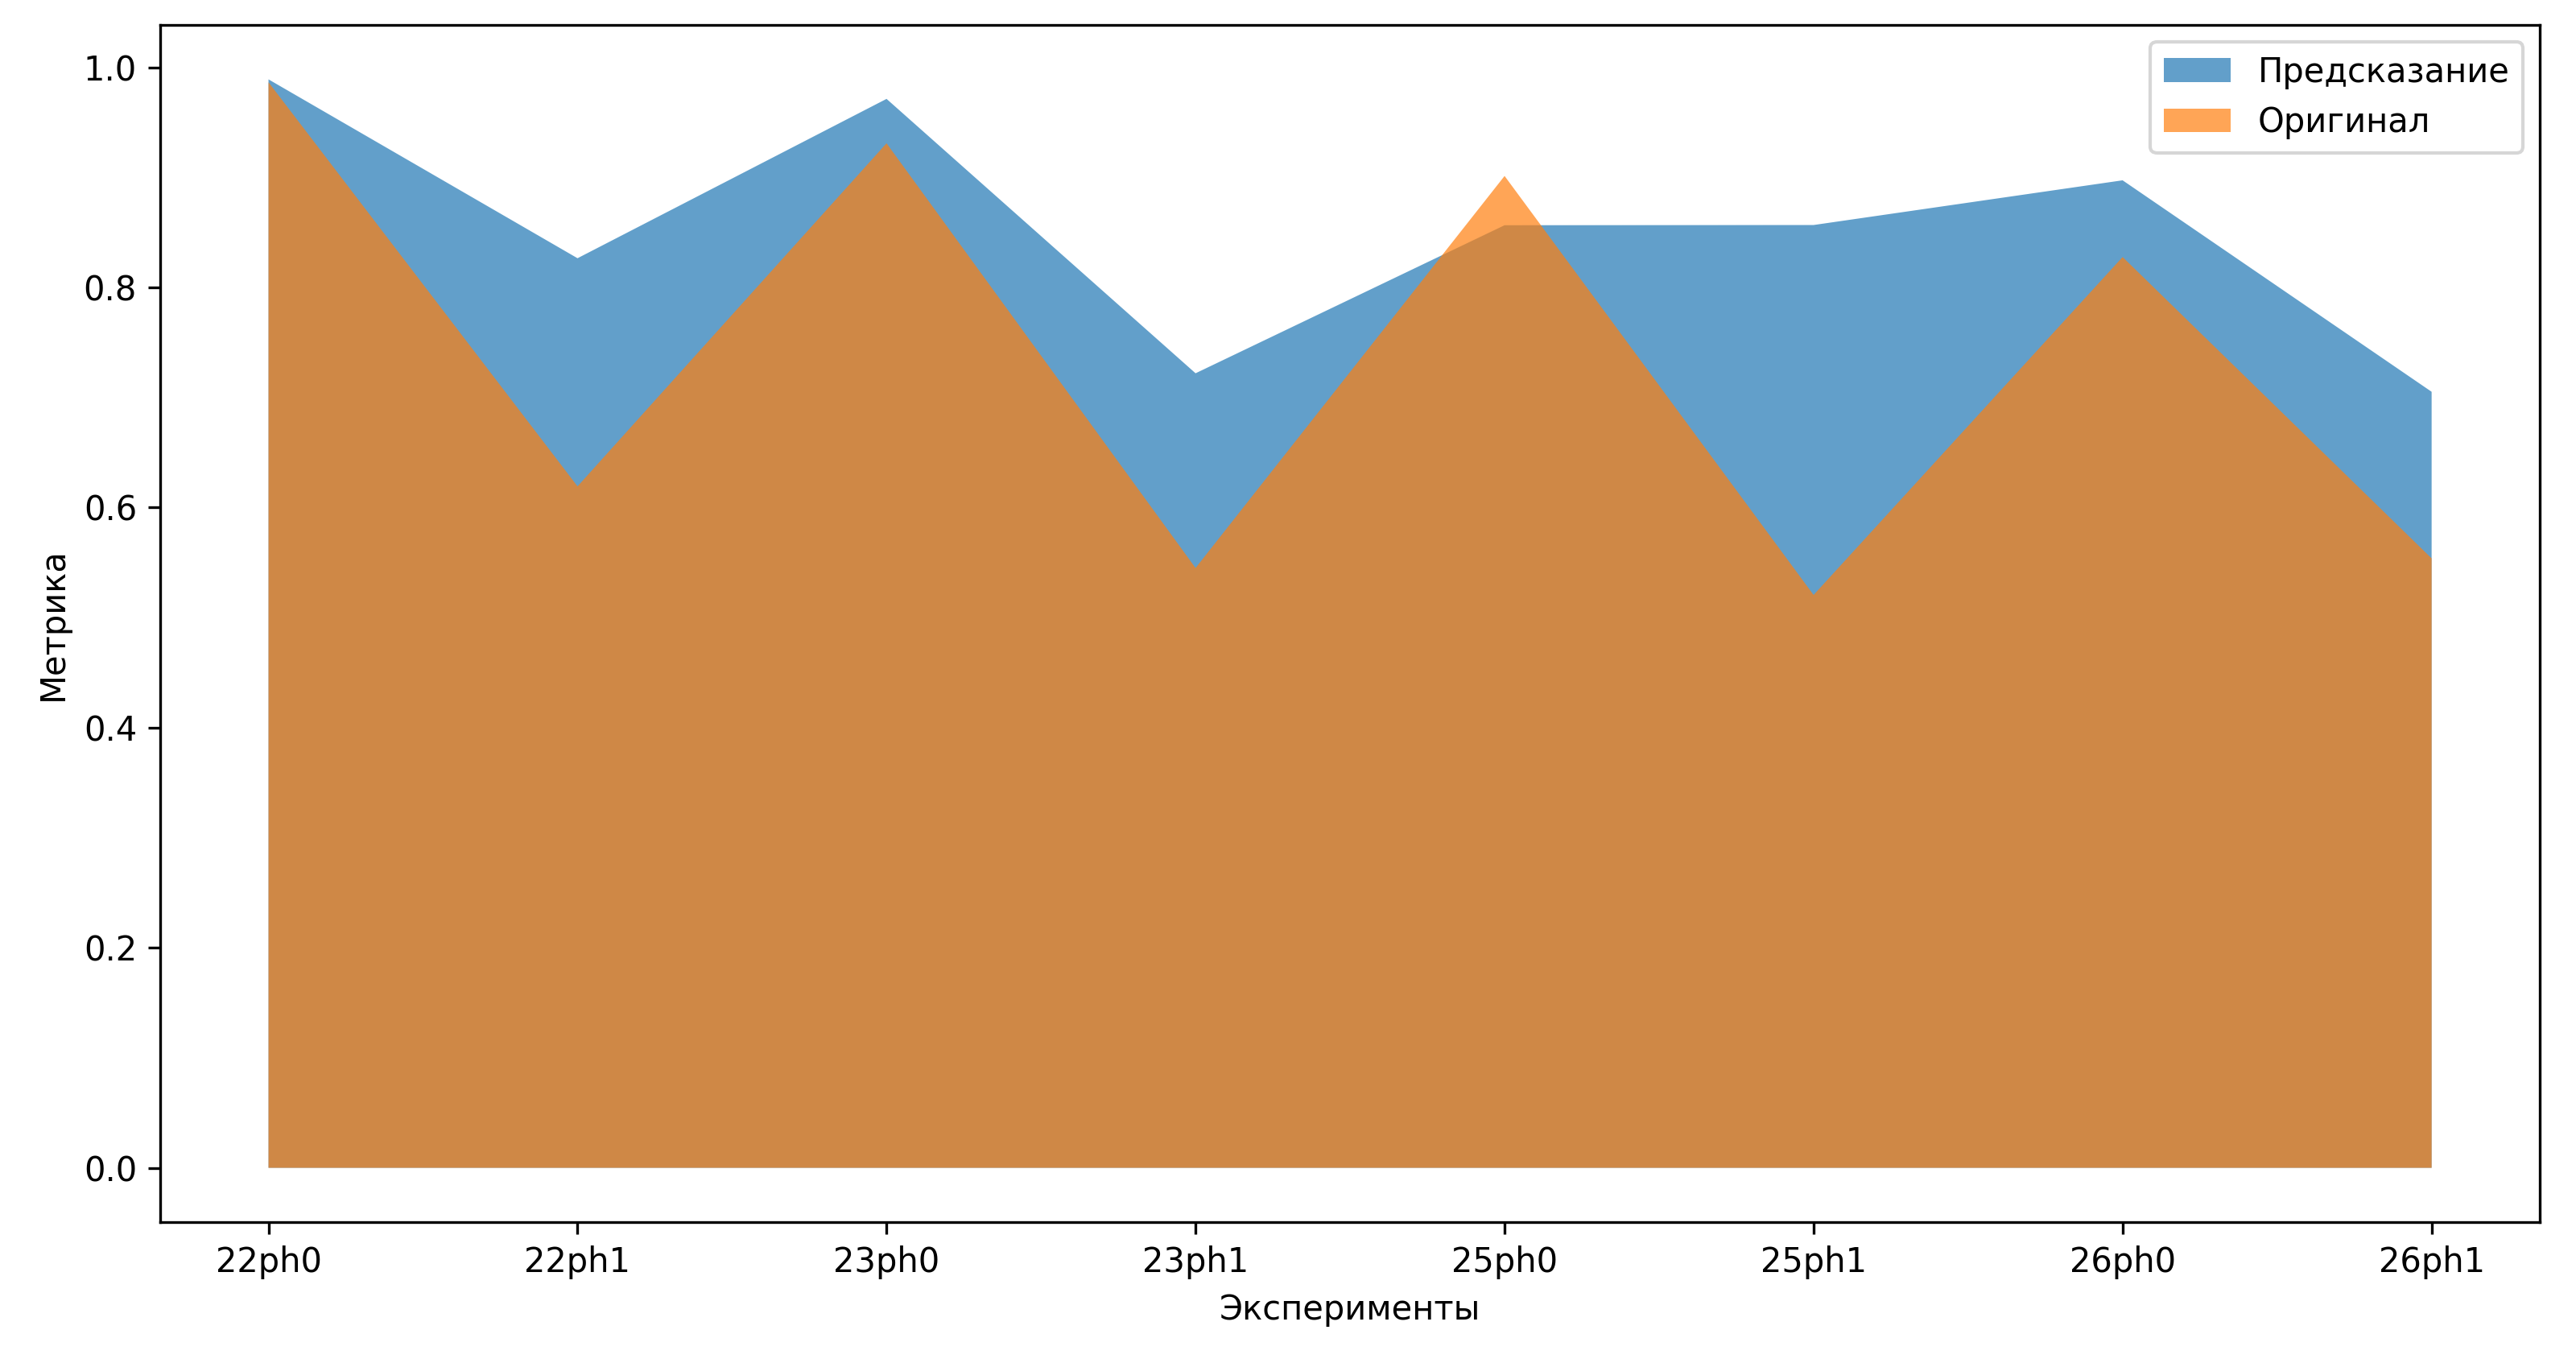
\includegraphics[width=\textwidth]{f1score-cropped.png}
	\caption{Сравнение F1-score оригинальной разметки и предсказанной}
	\label{fig:f1score-vs}
\end{figure}

Так же результат можно сравнить с альтернативным подходом, описанным в
\cite{anton}. У автора работы получилось достичь значения F1-score равным 0.83,
что чуть меньше, чем в данной работе (0.85). По большей части эта разница
достигается за счет использования более продвинутой архитектуры нейронной сети
UNet вместо SegNet.
